\documentclass[noback]{psuposter}

%%\documentclass[noback,portrait]{psuposter}
%% To make a poster in portrait, use the "portrait" option to
%% documentclass as shown above.

\usepackage{mathptmx}
\usepackage{xspace}
\usepackage{amsmath}
\usepackage{pifont}
\usepackage{psfrag}
\usepackage{wrapfig}
\usepackage{changepage}% has {adjustwidth}{<leftmargin>}{<rightmargin>} for tabbing in a column env.


%% Not needed for most posters %%%%%%%%%%%%%%%%%%%%%%%%%%%%
%%\renewcommand{\poster@ancimage}{/tmp/empty.ps}
\newcommand{\don}{\ensuremath{d_{\textsc{ON}}}}
\newcommand{\doff}{\ensuremath{d_{\textsc{OFF}}}}
\newcommand{\dsoma}{\ensuremath{d_{\textsc{SOMA}}} \xspace}
\newcommand{\um}{\ensuremath{\mu \text{m}}\xspace}
\newcommand{\dmin}{d$_{\textup{min}}$\xspace}
%%%%%%%%%%%%%%%%%%%%%%%%%%%%%%%%%%%%%%%%%%%%%%%%%%%%%%%%%%%


\begin{document}

%sensitive to length of title; may need to adjust font size
\title{\Huge One Approach for Evaluating the Ecological Sustainability of Agricultural Practices at the Landscape-scale}
%%\subtitle{The poster subtitle here}
\author{Bruce D. Marron$^1$}
\address{$^1$Portland State University, USA.}

\makeposter

\subsection{The Motivation}
\centerline{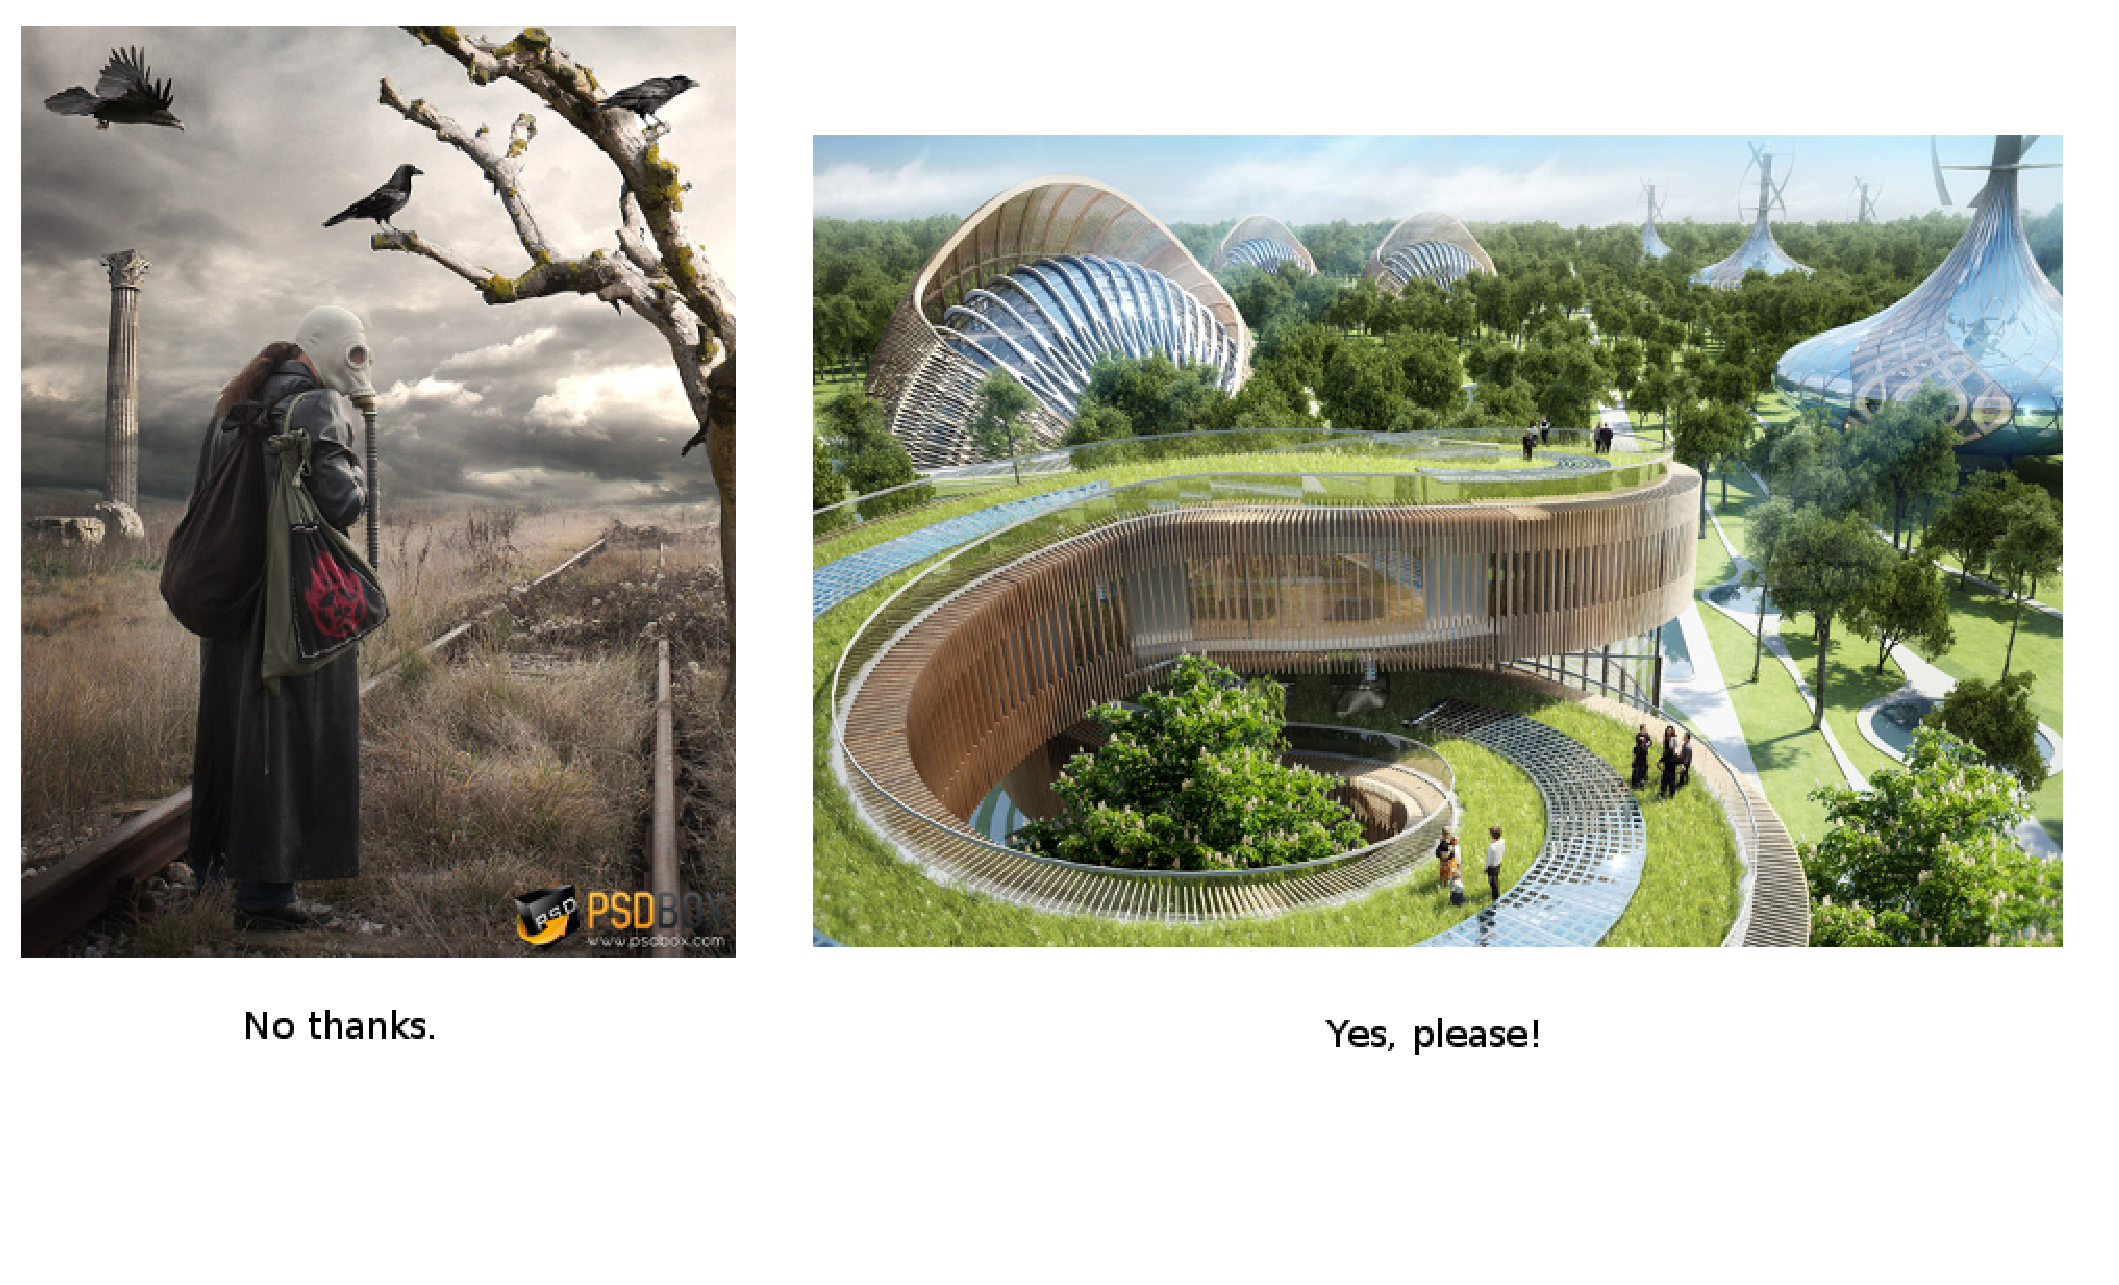
\includegraphics[width=20cm]{figs/Image1c.eps}}

Planetary-scale trends demand sustainable agriculture but no one knows what 'sustainable agriculture' really means or what it looks like at the landscape scale.  Bucket lists abound but a robust and flexible methodology for adequately differentiating agricultural practices with respect to their ecological impact is not available. This is because it is quite difficult to scientifically study the dynamics of the complex systems involved:  agro-ecological landscapes are coupled, complex adaptive systems that evolve in time and in space over multiple scales of both.
\subsection{The Questions}    
\begin{itemize}
\item How can we design robust and adaptive food production systems at a regionally-specific, landscape scale?
\item How can the dynamics of agro-ecological systems be used to develop synoptic keys for the classification of agricultural practices along the continuum of ecological resiliency? (Is a food production system ecologically sustainable or not?!)
\item What is the relationship between landscape-scale disturbance regimes, agricultural output, and biodiversity?
\item At any given time, which landscape mosaic is the 'most appropriate' one? How should we best manage succession and biodiversity at the landscape scale? 
\item How can we best monitor the state of ecological resources on a landscape? What are the (necessary and sufficient) state variables we need to assess the ecological health and resiliency of a given agro-ecological landscape pattern? 
\item How can we best use simulation to evaluate the ecological health and resiliency of new landscape pattern designs? 
\item What are the critical elements and processes shared by historical examples of both successful (e.g., \textit{milpa)} and disastrous (e.g., Dust Bowl) agro-ecological practices that can inform our transition to sustainable agriculture at the global scale?
\end{itemize}
\columnbreak
%
\subsection{The Proposed Methodology}
\centerline{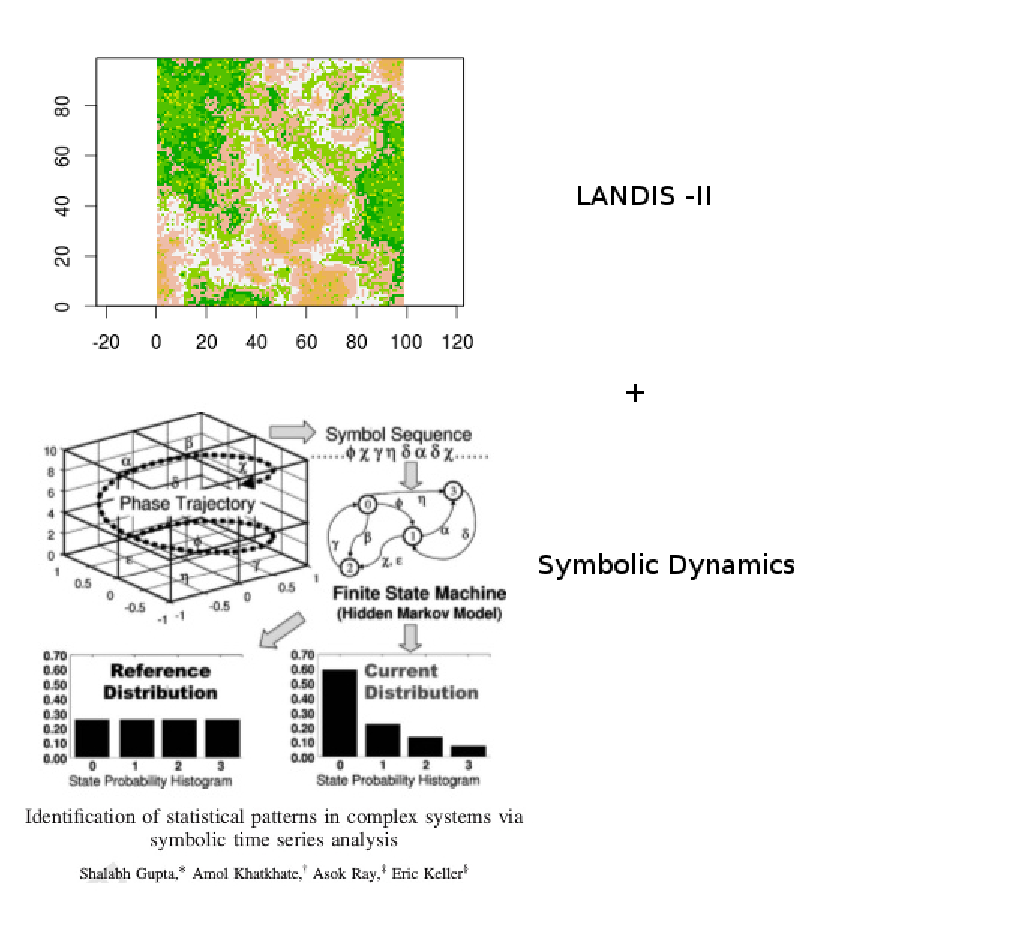
\includegraphics[height=15cm]{figs/Image2.eps}}
%
\subsection{The Proposed Heuristic}
%\vspace{-.5cm}
listening 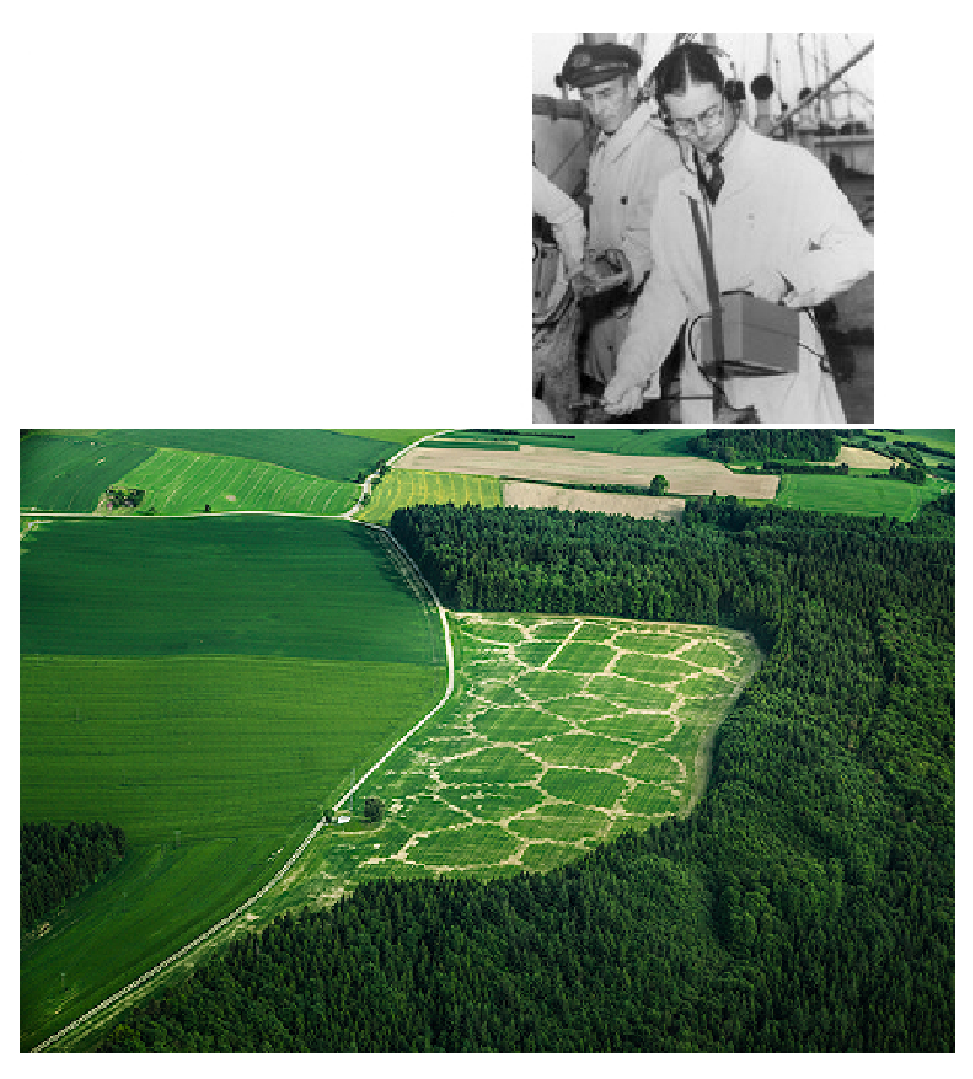
\includegraphics[height=7cm]{figs/Image3.eps}
\ plus \ 
\includegraphics[height=7cm]{figs/Image4.eps} 
translating (= aabbcdddd) \\ 
yields 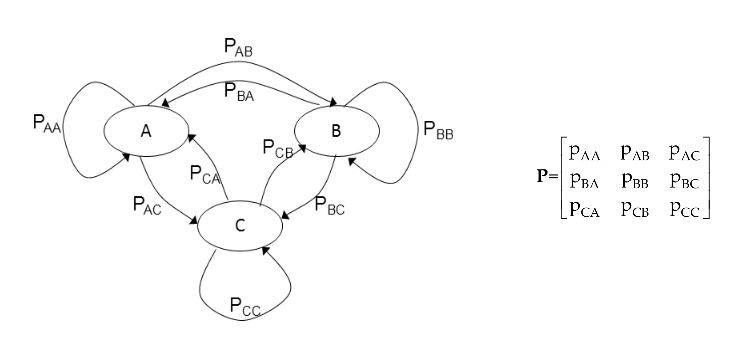
\includegraphics[height=8cm]{figs/Image5.eps}
\vspace{-1cm}
%
%
\subsection{The Proposed Algorithm}
%\vspace{-2cm}
\textbf{Level I: Build an m-dimensional vector of state variables.}
\begin{adjustwidth}{1cm}{}
{\small  Step 1. Select the set of key monitoring variables (KMVs).\\
Step 2. Fix the n-dimensional vector of required empirical variables (REVs).
}
\end{adjustwidth}
%\vspace{-.5cm}
\textbf{Level II: Define a set of landscape reference scenarios.}
%\vspace{-1cm}
\begin{adjustwidth}{1cm}{}
{\small Step 3a. Define five reference systems of human impact and presence on the landscape (so-called HIP classes) by differences in \% agriculture, \% forest, and \% built environment.\\
Step 3b. Define HIP subclass1 (conventional practices) and HIP subclass2 (agro-ecological practices).
}
\end{adjustwidth}
%\vspace{-.5cm}
\textbf{Level III: Translate the landscape reference scenarios to LANDIS-II.}
%\vspace{-1cm}
\begin{adjustwidth}{1cm}{}
{\small Step 4a. Given a specific landscape, define the ecoregions and the set of landscape patch-types for each of the reference systems under HIP subclass1 and HIP subclass2.\\
Step 4b. Provide each patch-type with a unique moniker, a unique MapCode, a list of species and their ages, and species attributes lists for building LANDIS-II files.\\
Step 5. Operationalize the LANDIS-II model for each of the HIP subclass reference systems. ("Operationalize" means to parameterize, calibrate (validate) and define the simulation settings for each model.)
}
\end{adjustwidth}
%\vspace{-.5cm}

\columnbreak

\textbf{Level IV: Build a landscape reference scenario codebook.}
\begin{adjustwidth}{1cm}{}
{\small Step 6. Perform multiple simulation runs for each of the HIP subclasses where each dataset will be a time series (t = 20) of the n-dimensional REVV. Transform all raw output data (REVVs) to KMVVs keeping time stamps intact.\\
Step 7. Define a set of unique landscape morphs (states) for each landscape reference scenario using a feature extraction method. Morphs will be derived from the collection of KMVVs generated by LANDIS-II. \\
Step 8a. Codify the morphs generated by each landscape reference scenario by giving each one a unique character symbol. \\
Step 8b. Compile the symbols, their prototype (reproduction) KMVVs, and their probability distributions into the complete landscape reference scenario codebook: the collection of Alphabet1 from HIP subclass1 plus Alphabet2 from HIP subclass2 (removing duplications).
}
\end{adjustwidth}
%
\textbf{Level V: Build m-order Markov chains (bigram models) for the reference landscape scenarios.}
\begin{adjustwidth}{1cm}{}
{\small Step 9. Apply the landscape reference scenario codebook to the original KMVV data set to obtain landscape morph time series data (sequences of symbols) for each reference scenario.\\
Step 10. Extract empirical frequencies from the time series data and use them to derive 1-step conditional probabilities. Use the derived conditional probabilities to define a bigram model for each scenario.
}
\end{adjustwidth}
%
\textbf{Level VI: Define agro-ecological sustainability for a given landscape.}
\begin{adjustwidth}{1cm}{}
{\small Step 11. Evaluate the ecological implications of the correlations evident in the transition (stochastic) matrices. \\
Step 12. Use ecological and biological principles to evaluate agro-ecological sustainability by examining the fluxes in the components of the KMVV relative to the sequence of morphs appearing over time.
}
\end{adjustwidth}
%
\textbf{Level VII: Evaluate the sustainability vocabulary of extant and novel landscape designs.}
\begin{adjustwidth}{1cm}{}
{\small Step 13. Ideally, define a landscape-specific, sustainability shift space where the "forbidden blocks" are thresholds in the stationary distribution of landscape morphs.
}
\end{adjustwidth}
\vspace{-1cm}
\subsection{Some Exploratory Efforts}
\vspace{-.5cm}
\small A simple experiment: (1) define a symbol generating system by a two-state, Markov chain (switching model); (2) use the switching model to simulate (Monte Carlo) a time series data set (t=1000); (3) extract the symbol frequencies in the simulated data to derive the bi-gram conditional probabilities; (4) use the ('empirically-derived') bi-gram probabilities to define the empirical symbol generating system; (5) compare the symbol generating systems (i.e., the known Markov chain to the empirically-derived Markov chain). For fun, try a bootstrap version!
\centerline{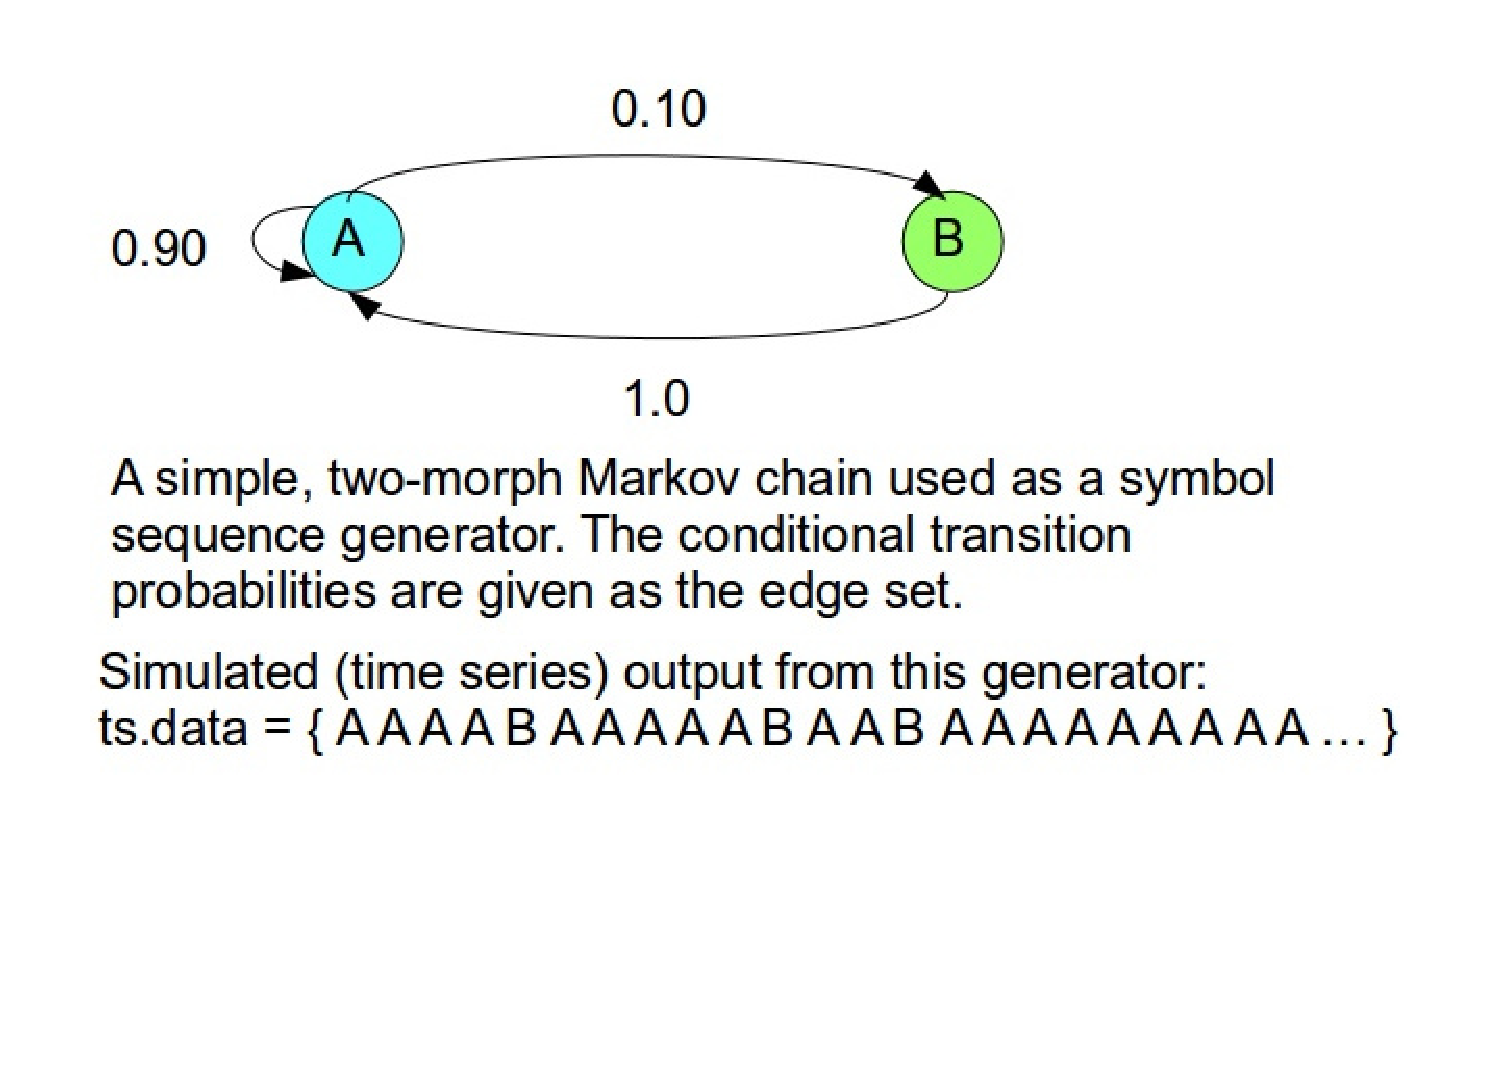
\includegraphics[height=12.5cm]{figs/Image6.eps}}
\vspace{-2cm}
{\scriptsize
\begin{verbatim}
G1 (known)         emp.G1 (MC sim.)       boot.emp.G1 (bootstrap)                Stat. Dist.       Rel. Entropy
     [,1] [,2]           [,1]  [,2]            [,1]   [,2]             known     [1] 0.909 0.091    0.000000
[1,]  0.9  0.1      [1,] 0.896 0.104      [1,]  0.908 0.092            MC sim.   [1] 0.906 0.094    0.000077
[2,]  1.0  0.0      [2,] 1.000 0.000      [2,]  0.974 0.025            bootstrap [1] 0.914 0.086    0.000230
\end{verbatim}
}
%


\end{document}

